\documentclass[10pt,fleqn]{article} % Default font size and left-justified equations
\usepackage[%
    pdftitle={Centrale Supelec 2018},
    pdfauthor={UPSTI}]{hyperref}

\input{style/new_style}
\input{style/macros_SII}
\usepackage{multicol}
\usepackage{siunitx}
%\usepackage{picins}
\fichetrue
%\fichefalse

\proftrue
\proffalse

\tdtrue
%\tdfalse

\courstrue
\coursfalse

% -------------------------------------
% Déclaration des titres
% -------------------------------------

\def\discipline{Sciences \\Industrielles de \\ l'Ingénieur}
\def\xxtete{Sciences Industrielles de l'Ingénieur}


\def\classe{\textsf{UPSTI}}
\def\xxnumpartie{CCS 2019}
\def\xxpartie{Chirurgie mini-invasive robotisée avec
stabilisation des mouvements physiologiques}

\def\xxnumchapitre{Concours Centrale Supelec}%Révision 1 \vspace{.2cm}}
\def\xxchapitre{PSI 2019}

\def\xxposongletx{2}
\def\xxposonglettext{1.45}
\def\xxposonglety{16}%16

\def\xxonglet{\textsf{CCS 2019}}

\def\xxactivite{TD 01}
\def\xxauteur{\textsl{UPSTI}}


\def\xxtitreexo{Chirurgie mini-invasive robotisée avec
stabilisation des mouvements physiologiques}
\def\xxsourceexo{\hspace{.2cm} \footnotesize{Concours Centrale Supelec PSI 2019}}

\def\xxcompetences{%
\textsl{%
%\textbf{Savoirs et compétences :}\\
}}

\def\xxfigures{
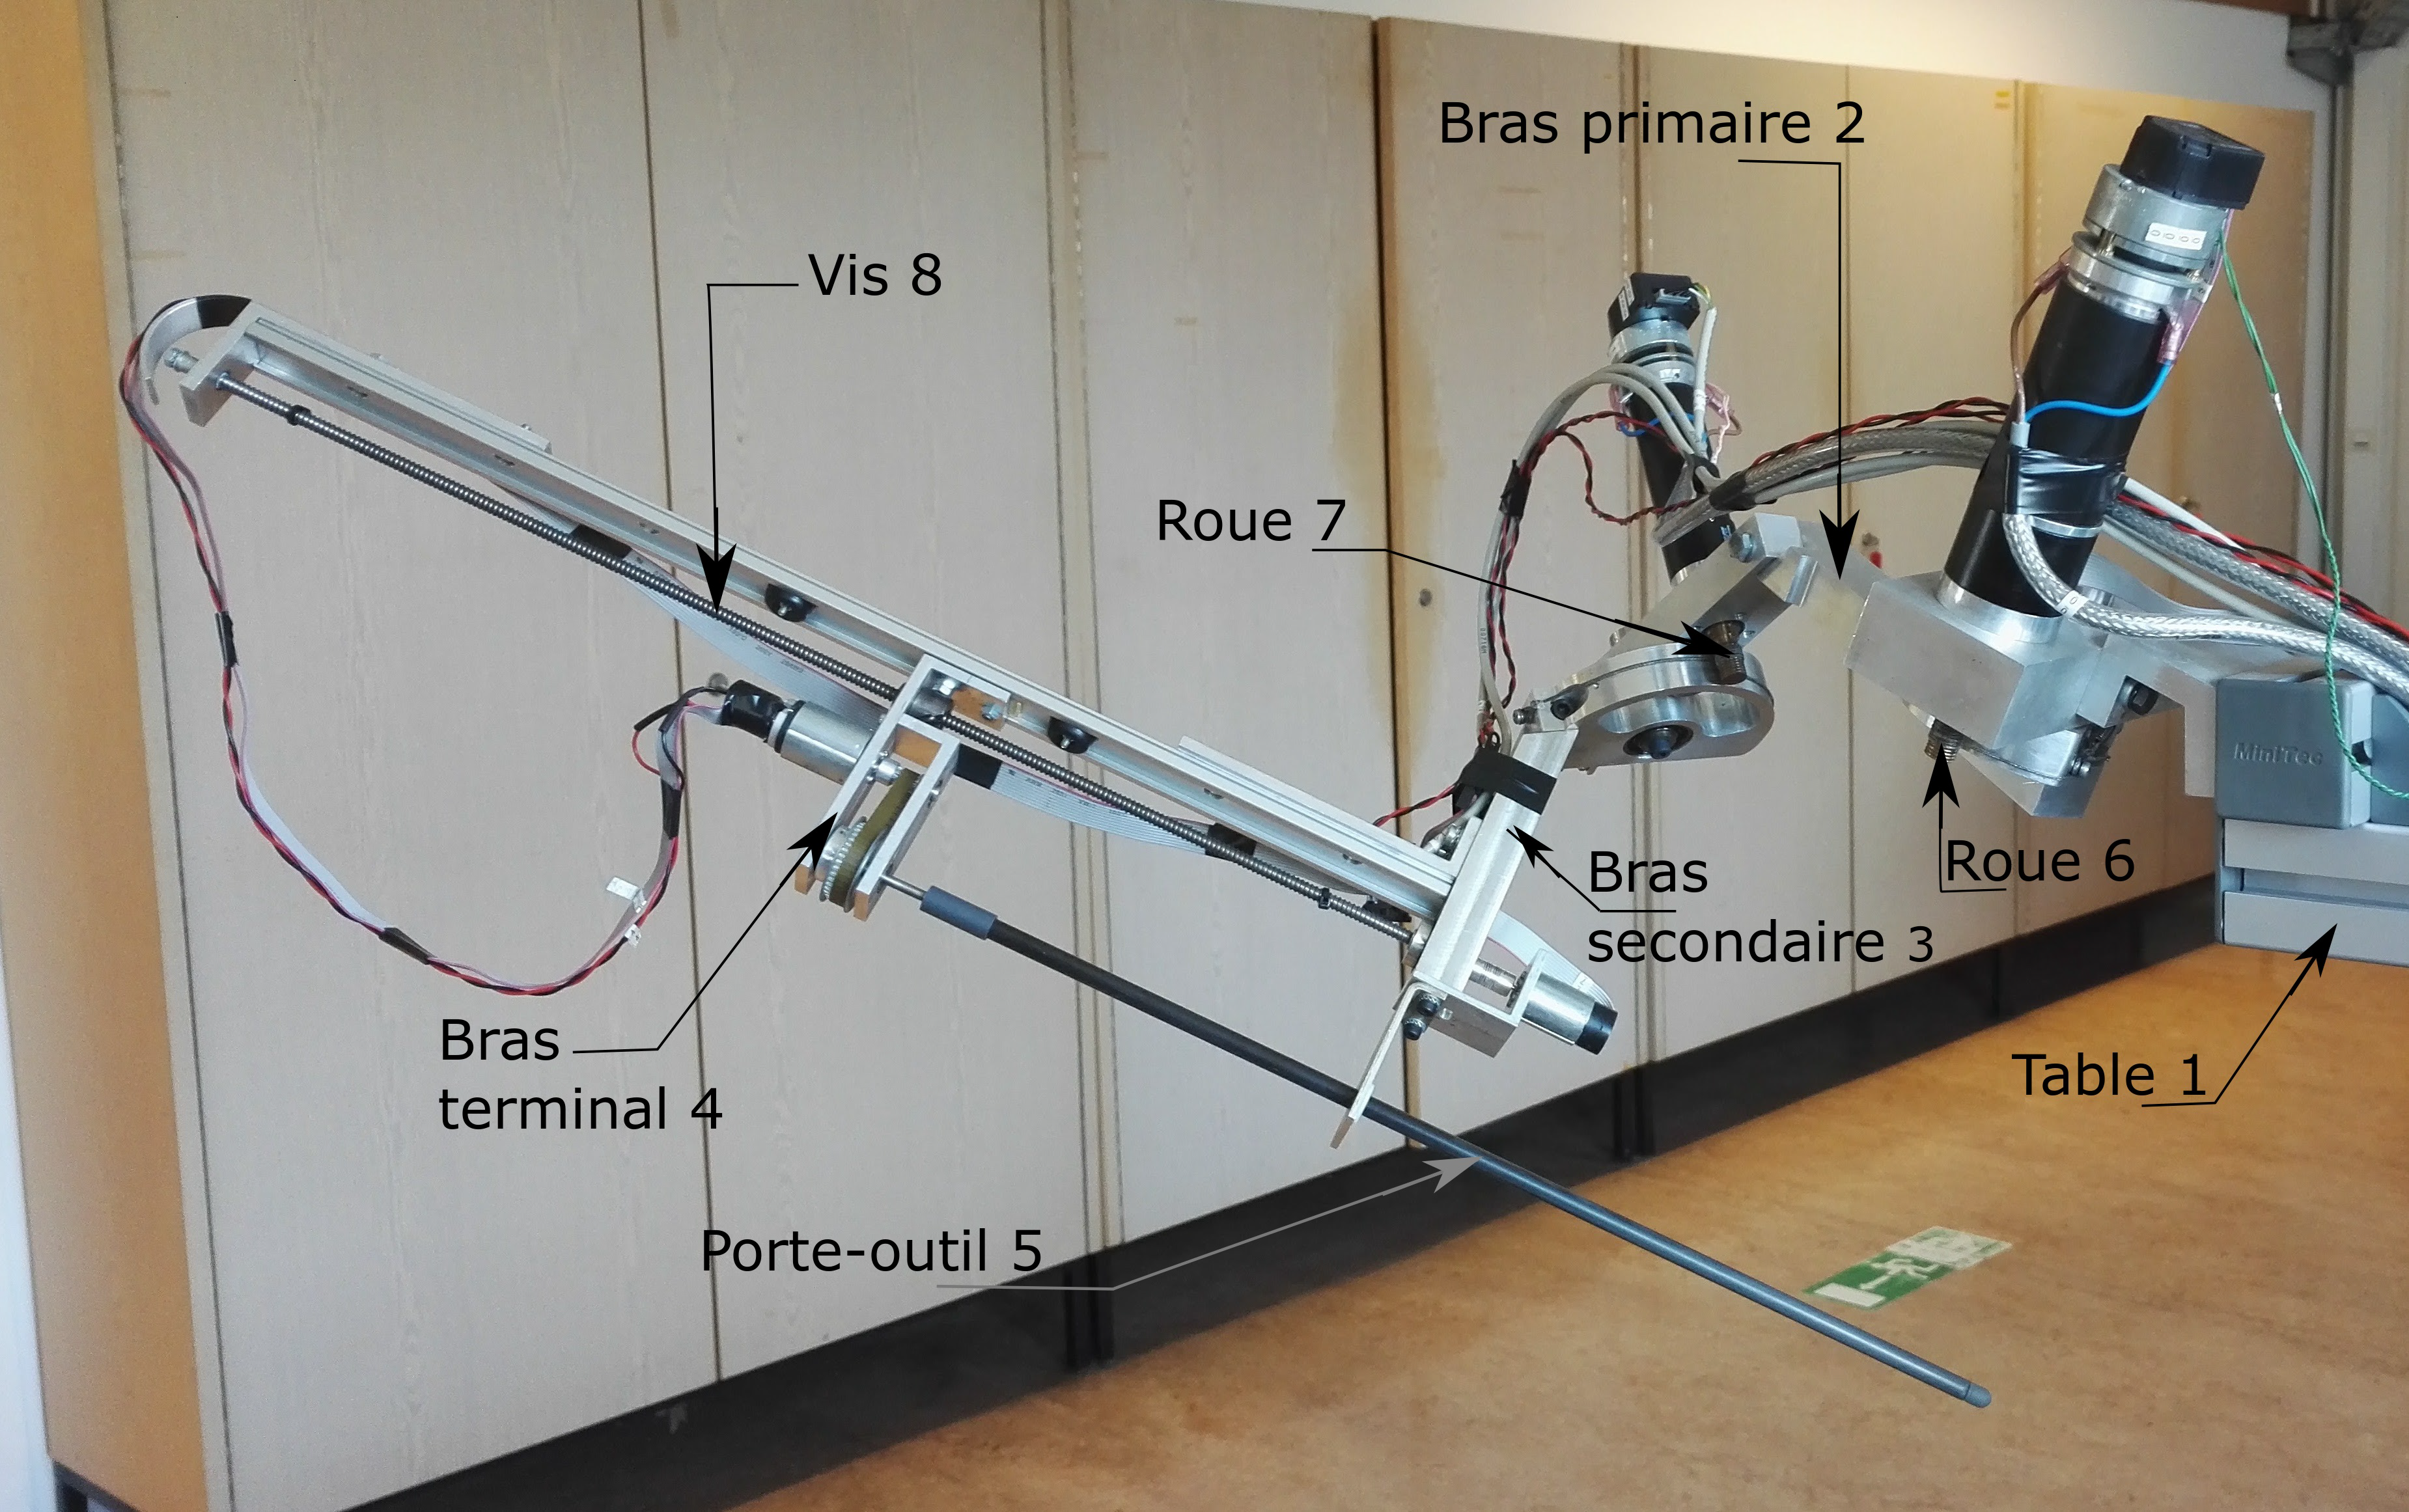
\includegraphics[width=.55\textwidth]{images/fig_00}
}%figues de la page de garde

\def\xxpied{%
Chirurgie mini-invasive robotisée\\
Concours Centrale Supelec -- PSI 2019%
}

\setcounter{secnumdepth}{5}
%---------------------------------------------------------------------------

\usepackage{bm}
\begin{document}
%\chapterimage{png/Fond_Cin}
\input{style/new_pagegarde}
\vspace{4.5cm}
\pagestyle{fancy}
\thispagestyle{plain}


\def\columnseprulecolor{\color{ocre}}
\setlength{\columnseprule}{0.4pt} 

\section{Analyse des propriétés des signaux physiologiques}

\begin{obj}
Analyser les propriétés des signaux physiologiques et en déduire des éléments du cahier des charges
de la loi de commande pour assurer le déplacement du robot avec le niveau de précision requis.
\end{obj}

\subsection{Analyse des propriétés des signaux des mouvements physiologiques}

\begin{obj}
Proposer un algorithme permettant de mettre en évidence les propriétés des mouvements respiratoires.
\end{obj}
\subparagraph{}
En première approximation, on peut dire que ce signal est périodique, de période \SI{4,8}{s}. La valeur maximale est de \SI{5}{mm} et la valeur minimale est de \SI{-2,5}{s}.
Si on avait à la modéliser par un signal sinusoïdal on aurait $e(t)=3,75 \sin\dfrac{2\pi}{4,8} t + 1,25$.

\subparagraph{}
D'après la définition, 
$\hat{S}\left( f_n\right)= \dfrac{1}{N_f} \sum \limits_{k=0}^{N_f-1} s\left[kT_e\right] \text{e}^{-i 2 \pi f_nT_e k}$

$= \dfrac{1}{N_f} \left(
 s\left[0 T_e\right] \text{e}^{-i 2 \pi f_nT_e 0} + 
 s\left[T_e\right] \text{e}^{-i 2 \pi f_nT_e } + ... 
 s\left[\left( N_f-1\right)T_e\right] \text{e}^{-i 2 \pi f_nT_e \left( N_f-1\right)}\right)$

$= \dfrac{1}{N_f} \left(
 s\left[0\right] + 
 s\left[T_e\right] \text{e}^{-i 2 \pi f_nT_e } + ... 
 s\left[\left( N_f-1\right)T_e\right] \text{e}^{-i 2 \pi f_nT_e \left( N_f-1\right)}\right)$.
 
 On a donc $l_k\left(f_n\right)=\dfrac{1}{N_f}\text{e}^{-i 2 \pi f_nT_e k}$.
 

\subparagraph{}

On a $L_n = \begin{pmatrix}  l_0 f_n  & l_1 f_n & l_2 f_n & \ldots & l_{N-1} f_n\end{pmatrix}$.
Par ailleurs, 
$S_p = 
\begin{pmatrix} \hat{S}\left( 0\right) \\ \hat{S}\left( f_1\right) \\ \hat{S}\left( f_2\right)  \\ \vdots \\ \hat{S}\left( f_{N-1}\right) \end{pmatrix} 
=
\begin{pmatrix} 
L_0 V_s \\
L_1 V_s \\
L_2 V_s \\
\vdots \\
 L_{N-1} V_s\end{pmatrix}$.

On a donc $ L_{k} V_s =\begin{pmatrix}  l_0 f_k  & l_1 f_k & l_2 f_k & \ldots & l_{N-1} f_k\end{pmatrix} \begin{pmatrix}
s[0]  \\ s[T_e] \\ s[2T_e] \\ \vdots \\ s\left[\left(N-1\right)T_e\right] \\   \end{pmatrix} = \sum  \limits_{i=0}^{N-1} l_i f_k s\left[i T_e\right]$.



\subparagraph{}

\subparagraph{}

\subparagraph{}

\subsection{Cahiers des charges partiel de la chaîne d'asservissement en position du robot esclave}

\begin{obj}
Déterminer une valeur numérique pour la bande passante de l’asservissement en position du robot
esclave et vérifier le cahier des charges associé.
\end{obj}

\subparagraph{}	

D'une part, $H(p)=\dfrac{\varepsilon (p)}{Z^*(p)}$ et d'autre part, $F(p)=\dfrac{Z (p)}{Z^*(p)}$. Enfin, $\varepsilon(p)=Z^*(p)-Z(p)$. On a donc $\varepsilon(p)=\dfrac{\varepsilon(p)}{H(p)} - F(p)Z^*(p)=\dfrac{\varepsilon(p)}{H(p)} - F(p)\dfrac{\varepsilon(p)}{H(p)}$. On a donc  $\varepsilon(p)=\dfrac{\varepsilon(p)}{H(p)} - F(p)\dfrac{\varepsilon(p)}{H(p)} \Leftrightarrow $ $H(p)=1 - F(p)= \dfrac{p^2+2\xi\omega_0 p }{p^2+2\xi\omega_0 p + \omega_0^2}$.


\subparagraph{}	


\subparagraph{}	


\section{Analyse géométrique et élaboration du modèle dynamique du robot esclave}

\begin{obj}
Vérifier la capabilité du robot esclave à respecter le cahier des charges et déterminer le modèle dynamique
d’un des axes du robot esclave utilisé pour dimensionner sa commande.
\end{obj}

\subsection{Vérification de la capabilité du robot esclave}
\begin{obj}
Vérifier la capacité du robot esclave à respecter l’exigence de précision 1.3.3 et dimensionner les
capteurs installés sur le robot en conséquence.
\end{obj}


\subparagraph{}%10	
\subparagraph{}%11
On a $\lambda(t)=\lambda_0 + \dfrac{p}{2\pi} \theta_{83}$. 
En conséquences, $\vect{BD}=\vect{BC}+\vect{CD}=l_3\vect{y_3}+\lambda(t)\vect{z_3}+l_4\vect{z_4}
=l_3\vect{y_3}+\left( \lambda_0 + \dfrac{p}{2\pi} \theta_{83} \right)\vect{z_3}+l_4\vect{z_3}$.


\subparagraph{}%12
En projetant $\vect{BD}$ dans la base $\base{x_2'}{y_2'}{z_2'}$, on a 
 $\vect{BD}=l_3\vect{y_3}+\left( \lambda_0 + \dfrac{p}{2\pi} \theta_{83} \right)\vect{z_3}+l_4\vect{z_3}$
 $ =l_3\left( \cos \theta_{32} \vect{x_2'} + \sin\theta_{32} \vect{y_2'}  \right)+\left( \lambda_0 + \dfrac{p}{2\pi} \theta_{83} +l_4\right)\vect{z_2'}$.
 
 Avec l'hypothèse que $\theta_{32}$ reste petit, on a  $\vect{BD}=l_3\left(  \vect{x_2'} + \theta_{32} \vect{y_2'}  \right)+\left( \lambda_0 + \dfrac{p}{2\pi} \theta_{83} +l_4\right)\vect{z_2'}$.
 
  Ainsi, $\left(x_D,y_D,z_D\right)=
\left( l_3,l_3 \theta_{32}, \lambda_0 + \dfrac{p}{2\pi} \theta_{83} +l_4\right)$.

\subparagraph{}%13

\subsection{Détermination et vérification du modèle dynamique du robot esclave}
\begin{obj}
Déterminer le modèle dynamique du robot esclave en vue de l’élaboration de sa commande.
\end{obj}

\subparagraph{}%14
\subparagraph{}%15
\end{document}

\subparagraph{}\textit{}


\begin{center}
\includegraphics[width=\linewidth]{images/img_04}
%\textit{}
\end{center}



